\chapter{Komponenter}
\label{komponenter}

\section{Resistorn}
 \textbf{HAREC a.\ref{HAREC.a.2.1}\label{myHAREC.a.2.1}}
\index{resistor}
\index{resistans}

\subsection{Allmänt}

Strömkretsar består av komponenter med olika egenskaper.
Den vanligaste egenskapen, åtminstone i likströmskretsar,
är resistansen.  För att få avsedd funktion, så anpassar
man resistansen i komponenterna.

\noindent\textbf{Exempel}: En krets med strömkälla, lampa,
kopplingsledningar och smältsäkring.

Kopplingsledningarna mellan komponenterna bör ha låg
resistans och därför lågt spänningsfall (små förluster).
Lampan ska däremot ha hög resistans och därmed höga
förluster för att kunna bli het och lysa.
Smältsäkringen ska skydda ledningarna från för hög ström.
Säkringen ges därför en resistans som gör att den smälter när strömmen
överstiger ett tillåtet värde.

Som hjälpmedel för att fördela spänningar och strömmar i en krets används
en komponenttyp kallad \emph{resistor}.
Dess utmärkande egenskap är \emph{resistans} (eng. \emph{resistance}) --
även kallad ohmskt motstånd.

\subsection{Enheten ohm}
\textbf{HAREC a.\ref{HAREC.a.2.1.1}\label{myHAREC.a.2.1.1}}
\index{ohm (\(\Omega\))}
\index{enheter!ohm (\(\Omega\))}
\index{symbol!\(R\) resistans}

(Se även kapitel \ref{ellära}.)

Resistansen mellan två punkter i en strömkrets är
\SI{1}{\ohm} som även skrives \SI{1}{\ohm} (uttalas ''en
åm''), när spänningen \SI{1}{V} mellan punkterna gör att
en ström av \SI{1}{A} (en ampere) flyter i kretsen.

Inom elektroniken används höga resistansvärden och därför även följande
multipler av enheten:

\begin{table}[h]
  \begin{tabular}{lll}
    1 kiloohm & \SI{1}{\kilo\ohm} & = \SI{1d3}{\ohm} \\
    1 megaohm & \SI{1}{\mega\ohm} & = \SI{1d6}{\ohm} \\
  \end{tabular}
  \caption{Motståndsvärden och deras relationer}
\end{table}

\subsection{Resistans i strömledare}
\textbf{HAREC a.\ref{HAREC.a.2.1.2}\label{myHAREC.a.2.1.2}}
\index{resistivitet}
\index{specifik resistans}
\index{symbol!\(\rho\) resitivitet}

För att bestämma resistansen i exempelvis en tråd, behöver man veta dess 
resistivitet, tvärsnittsyta, längd och temperatur.

\emph{Resistivitet} (eng. \emph{resitivity}) är ett materials
strömledningsegenskaper.
Ett annat namn för resistivitet är \emph{specifik resistans}.
Symbolen för resistivitet är \(\rho\) (uttalas ''rå'').

Formeln for resistivitet är:
\[
	\rho = \frac{R A}{l} \left[\frac{\unit \cdot \unit{mm^2}}{m}\right]
\]

där resistansen \(R\) på en längd \(l\) av en strömledare med en
genomsnittsarea \(A\) (som oftast anges i kvadratmillimeter).

Resitiviteten för material finns ofta i tabeller, och i bilaga
\ref{metallersresitivitet} finns ett antal vanliga metallers resitivitet
angivna.

Följande formel gäller för beräkning av resistansen i en strömledare med
linjär ström/spänningskaraktär.

\[R = \rho \dfrac{l}{A}\]
Där:
\[ 
	l\unit{[m]} \qquad A\unit{[mm^2]} \qquad \left[\rho = \frac{\Omega \cdot A}{m} \right] 
\]

\textbf{Exempel}

\(l = 4\ m\) koppartråd med arean \(A = 2\ mm^2\) ger oss \(\rho \text{ (koppar)} = 0,017\).
\[
R = \dfrac{\rho \cdot l}{A} \qquad \rightarrow \qquad R = \dfrac{0,017 \cdot 4}{2} = 0.034\ \Omega
\]
\marginnote{Not. Förväxla inte \(A\) som här är tvärsnittsytan i denna formel med enheten ampere. Bokstaven \(A\) kan nämligen betecka både storheten area och enheten ampere.}

\subsection{Resistiva material}

Resistorer kan utföras med olika typer av resistiva material, vilket bestämmer
användningsområdet. En resistor, vars resistans är oberoende av ström, spänning
och annan yttre påverkan t.ex. temperatur och ljus, sägs ha linjär karaktär.
Om resistansen däremot beror av yttre påverkan, så sägs resistorn ha olinjär
karaktär. 

Man skiljer mellan tre huvudgrupper av resistiva material. Det kan
vara en kropp av pressat kol eller ett ledande ytskikt på ett isolerande
underlag eller metalltråd på en isolerande stomme. 

På senare tid har det
tillkommit resistornät med integrerade resistorer, dvs. flera resistorer av
resistiva skikt på ett gemensamt isolerande underlag. Här beskrivs i korthet
olika typer av resistorer.

\subsection{Utförandeformer}

Resistorer kan utföras med fast eller ställbart resistansvärde. Här följer
först en översikt över resistorer med olika resistiva material och fast
resistansvärde.

\subsection{Fasta resistorer med linjär karaktär}

\subsubsection{Massaresistor}
\index{massaresistor}
\index{resistor!massa-}

Det resistiva materialet består av kolmassa med bindemedel (kolkomposit).
Massan är bakad till en stav eller ett rör. Anslutningsledningarna är inbakade
i materialet.
\emph{Massaresistorer} är lämpliga för lik- och växelströmskretsar med
låga krav på temperaturberoende och egenbrus. Den homogena kroppen gör att
egeninduktansen är låg. Å andra sidan uppstår vid höga frekvenser en skineffekt, 
det vill säga en strömkoncentration vid ytan, som medför viss resistansökning.

\subsubsection{Kolfilmsresistor}
\index{kolfilmresistor}
\index{resistor!kolfilm-}

Det resistiva materialet består av ett kolskikt, som genom förångning överförts
till ett keramiskt rör.
Resistansen bestäms av tjockleken på skiktet samt av spiralformade spår i
detta.
Genom spiraliseringen tillförs en induktans, som dock i någon mån uppvägs av
egenkapacitansen.

\subsubsection{Metallfilmresistor}
\index{metallfilmresistor}
\index{resistor!metallfilm-}

I denna typ är kolfilmen ersatt av ett metallskikt.
Eftersom egenkapacitansen är liten är typen lämpad för höga frekvenser.

\subsubsection{Tjockfilmsresistor}
\index{tjockfilmsresistor}
\index{resistor!tjockfilm-}

Det resistiva materialet består av en film av bland annat metalloxid, som screentrycks
på ett keramiskt underlag. Typen har god tålighet mot pulser och höga
temperaturer, men har relativt högt egenbrus.
Ytmonterade resistorer är oftast tillverkade av tjockfilm.

\subsubsection{Tunnfilmsresistor}
\index{tunnfilmresistor}
\index{resistor!tunnfilm-}

Det resistiva materialet består av en tunn metallfilm, som genom förångning
överförts till ett underlag av glas eller keramik. Denna resistortyp har över
lag god stabilitet och används ofta i apparater med hög precision.
Egenskaperna vid höga frekvenser är dock inte så goda.

\subsubsection{Metalloxidresistor}
\index{metalloxidresistor}
\index{resistor!metalloxid-}

Denna resistortyp har ett spiralformat skikt av metalloxid.
Temperatur- och spänningsberoendet är måttligt.
Tåligheten mot pulser och höga temperaturer är stor.
Typen kan i någon mån ersätta trådlindade resistorer.

\subsubsection{Resistornät}
\index{resistornät}
\index{resistor!-nät}

Resistornät (integrerade resistorer) består av flera resistiva skikt på ett
gemensamt isolerande underlag, det vill säga en liknande teknik som för tjock- 
och tunnfilmsresistorer.

\subsubsection{Trådlindad resistor}
\index{trådlindad resistor}
\index{resistor!trådlindad}

Det resistiva materialet är en metalltråd lindad på en stomme som tål
hög temperatur. Stommen kan vara av keramik, glas eller liknande.
Tåligheten mot pulser och höga temperaturer är stor.

\subsection{Fasta resistorer med olinjär karaktär}
\textbf{HAREC a.\ref{HAREC.a.2.1.3}\label{myHAREC.a.2.1.3}}
\index{olinjära resistorer}
\index{resistor!olinjär}

Vanligast är att materialet i resistorer har linjär ström- och spänningskaraktär,
men det finns även sådana med olinjär karaktär. I resistorer med olinjär
karaktär är det ingående materialet av halvledartyp.

\subsubsection{Spänningsberoende resistor --- Voltage Dependent Resistor (VDR)}
\index{spänningsberoende resistor}
\index{resistor!spänningsberoende}
\index{VDR}
\index{resistor!VDR}

Linjära resistorer påverkas knappast av den pålagda spänningen.
Resistorer av kiselkarbid har däremot en hög resistans vid låg spänning och
omvänt en låg resistans vid hög spänning.
Sådana spänningsberoende resistorer används till exempel för begränsning av
spänningstoppar.

\subsubsection{Ljusberoende resistor, fotoresistor --- Light Dependent Resistor (LDR)}
\index{ljusberoende resistor}
\index{resistor!ljusberoende}
\index{fotoresistor}
\index{resistor!foto-}
\index{LDR}
\index{resistor!LDR}

Ledningsförmågan i halvledare påverkas inte bara av värme utan även av ljus.
Halvledare av germanium och särskilt sammansatta halvledare av kadmiumoxid,
blysulfid och indiumantimonid har särskilt stor ljuskänslighet. Kadmiumsulfid
är känsligast för synligt ljus medan andra material är känsligast i det
infraröda området.

\subsubsection{Magnetfältberoende resistor (fältplatta)}
\index{magnetfältberoende resistor}
\index{resistor!magnetfältberoende}
\index{hallresistor}
\index{resistor!Hall-}

Resistansen ökar med längden på strömledaren. Denna egenskap används i
\emph{magnetfältsberoende fältplattor} som utnyttjar \emph{halleffekten}, även
kända som \emph{hallresistor}. En sådan består av en keramisk bärarplatta med
en yta av indiumantimonid. I ytan är ytterst smala parallella metallbanor
inlagda på ett avstånd av någon \textmu m (mikrometer). Normalt går strömmen kortaste vägen
tvärs över banorna, men när ett magnetfält träffar vinkelrätt mot plattans yta,
så avlänkas elektronerna. De får då längre väg över till nästa metallbana och
den totala resistansen ökar.

\subsubsection{Temperaturberoende resistor}
\index{temperaturberoende resistor}
\index{resistor!temperaturberoende}
\index{NTC}
\index{resistor!NTC}
\index{PTC}
\index{resistor!PTC}

Se nedan om NTC och PTC i resistorer.

\subsection{Temperaturkoefficienten för resistorer}
\index{temperaturkoefficient i resistor}
\index{resistor!temperaturkoefficient}
\index{NTC}
\index{resistor!NTC}
\index{PTC}
\index{resistor!PTC}

Resistansen i ingående material påverkas av temperaturen, varvid det skiljer
mellan materialen.

Amorft kol och de flesta halvledande material leder bättre när de är varma --- de
har en negativ temperaturkoefficient (NTC). Sådana material finns t.ex. i
dioder och transistorer.

Däremot leder metaller och speciella halvledarmaterial bättre när de är kalla
--- de har en positiv temperaturkoefficient (PTC). Glödtråden i glödlampor och
elektronrör är resistorer med positiv temperaturkoefficient (PTC). I vissa
metallegeringar, som t.ex. i konstantan, kan resistansen till och med vara
nästan konstant vid varierande temperatur.

Alla material har en temperaturkoefficient, som anger hur mycket resistansen
ändras per grad. Resistansen vid någon annan temperatur kan därför beräknas med
följande formel, där man sätter in begynnelsetemperaturen [ \(\vartheta\) ]
(\degree C), temperaturändringen [\(\Delta \vartheta\)] och
temperaturkoefficienten [\(\alpha\)].
\[R_{varm} = R_{kall} \pm \alpha \cdot \Delta \vartheta \cdot R_{kall}
\]

Resistansändringen är ledet

\[\Delta R = \pm \alpha \cdot \Delta \vartheta \cdot R_{kall}
\]
Temperaturkoefficienten kan vara positiv (PTC) eller negativ (NTC).
I principscheman har PTC- respektive NTC-resistorer symboler som på bilden.

\begin{figure}
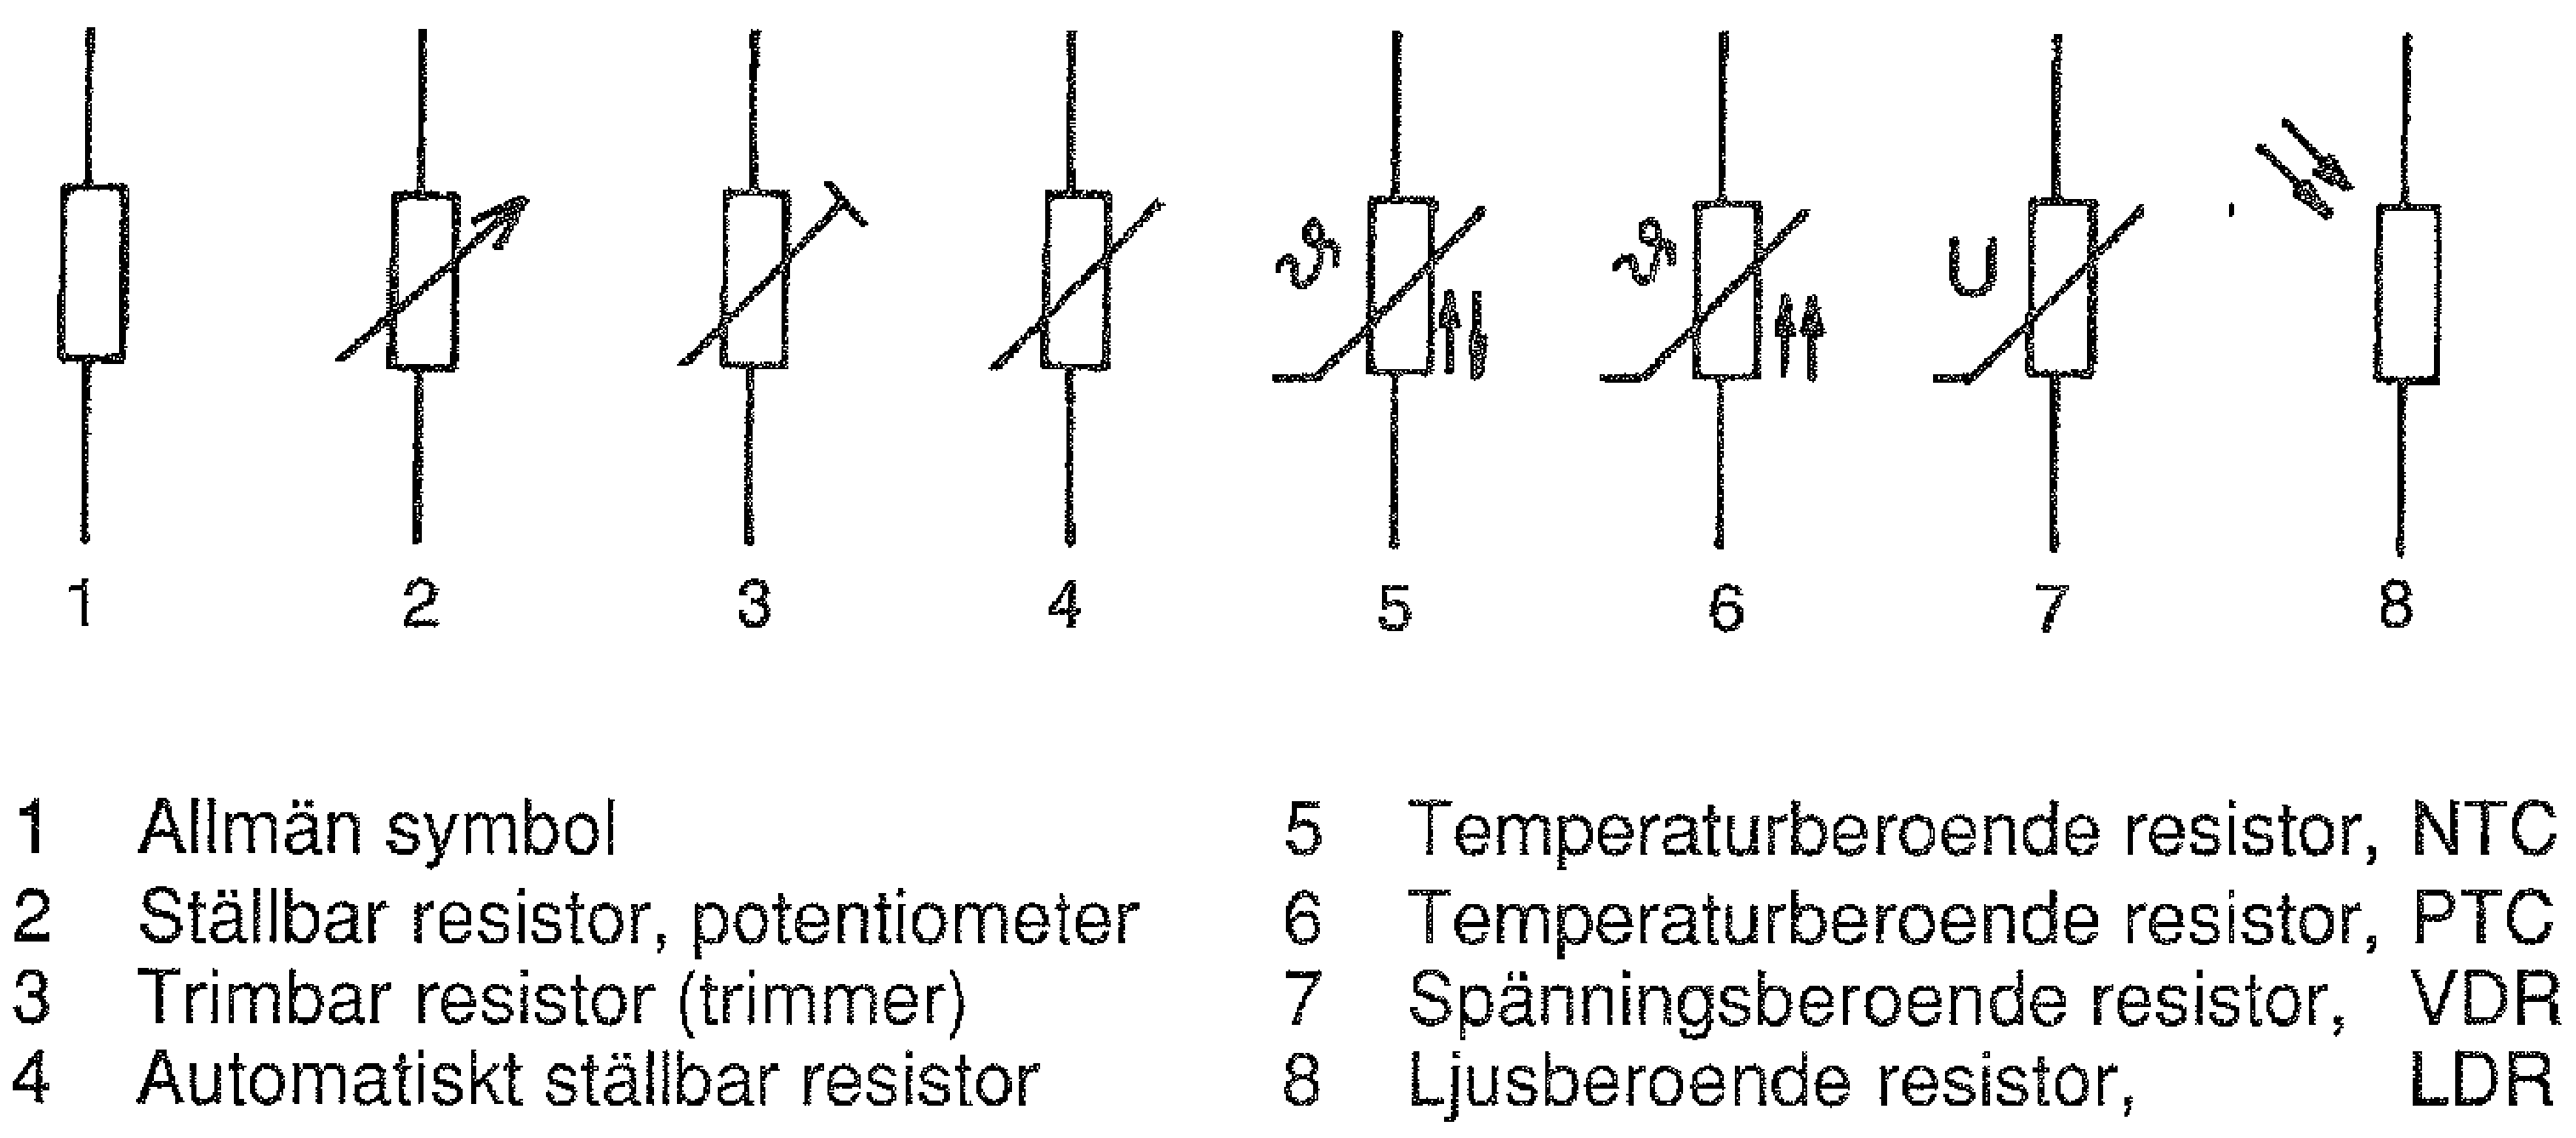
\includegraphics[width=\textwidth]{images/cropped_pdfs/bild_2_2-01.pdf}
\caption{Schemasymboler för resistorer}
\label{fig:BildII2-1}
\end{figure}

\subsection{Variabla resistorer}
\index{variabla resistorer}
\index{resistor!variabel}

En resistor kan även utföras med variabelt resistansvärde. Då används endast
den andel av det resistiva materialet som finns mellan en resistors ena ände
och ett uttag någonstans mellan ändarna. En sådan anordning kallas för reostat.
Om en variabel resistor används som spänningsdelare kallas den för
potentiometer.

I en potentiometer används dels hela resistansen mellan ändpunkterna och dels
andelen mellan uttaget och någon av ändpunkterna. Uttagets mekaniska utförande
beror oftast av hur bekvämt inställningen ska kunna ske. En potentiometer,
där det resistiva materialet är lagt på en cirkulär bana och uttaget är fäst
vid en axel i banans centrum, medger enkel inställning med mejsel, ratt eller liknande.
Ett enklare slags uttag är en släpkontakt eller ett spännband som kan flyttas
utmed en stavformad resistor.

\subsubsection{Resistiva material i variabla resistorer}

Banan i en variabel resistor består i princip av liknande resistiva material
som i en fast resistor. Billigast och enklast är en bana av kol, som är tryckt
på ett enkelt underlag. Nackdelar är låg effekttålighet, dålig upplösning och
linjäritet, högt brus och kort livslängd. Fördelen är lågt pris.
Bättre än en kolbana är en bana av kolkomposit, det vill säga kolpulver med 
bindemedel, som är tryckt på ett underlag. Nackdel är högre pris och låg 
effekttålighet, medan fördelarna är god upplösning, lågt brus och lång livslängd.
Vill man ha god effekttålighet och temperaturstabilitet, utöver kolkompositens
egenskaper, så erbjuder en bana av cermet sådana fördelar. En cermetbana består
av en blandning av metaller och keramik, som trycks på ett underlag.
Trådlindad bana har främst god tålighet mot hög effekt. Tålighet vid hög ström
genom uttaget är en annan fördel.

\subsubsection{Linjära och olinjära potentiometrar}

En potentiometers resistansändring som funktion av uttagets rörelseväg utmed 
resistansbanan kan beskrivas med en kurva. Kurvformen kan utföras linjär,
logaritmisk, eller på något annat sätt. Olinjära kurvor består oftast av en följd av 
linjära segment, som tillsammans någorlunda motsvarar den önskade olinjära 
formen.

\subsection{Effektutveckling i resistorer}
\textbf{HAREC a.\ref{HAREC.a.2.1.4}\label{myHAREC.a.2.1.4}}
\index{effektutveckling i resistorer}
\index{resistor!effektutveckling}

I resistorer utvecklas värme av den ström som flyter igenom dem. Värmeutvecklingen
sker enligt Joules lag, som återges i kapitel \ref{ellära}. Hur mycket effekt i form av
värme som strålas ut från resistorn beror på storleken på dess yta och
egentemperatur samt på omgivningens temperatur. Det finns en övre gräns för hur
mycket värme det ingående materialet tål innan det förstörs och eventuellt fattar
eld. En resistors effekttålighet framgår i vissa fall av påstämplade värden.
I övriga fall är man hänvisad till kataloguppgifter eller en bedömning, som
eventuellt kan grundas på höljets utseende och dimensioner.

\subsection{Standardiserade komponentvärden}
\index{resistor!standardiserade värden}

Resistorer tillverkas vanligen med standardiserade värden från en talserie.

\subsection{Märkning av resistorer}

Resistorer märks med hjälp av siffror och bokstäver eller med en färgkod så att
resistorns huvuddata kan avläsas. Ofta finns märkningen förklarad i 
komponentleverantörenas kataloger.
